\begin{minipage}[t]{0.7\textwidth}
	Une étape d'analyse du code (parsing) est nécessaire en amont de la production du code assembleur. Cette étape a pour objet:
\begin{itemize}
	\item d'assurer que la syntaxe du langage jouet est respectée
	\item de permettre la construction d'un arbre représentant les différentes structures du code source afin de pouvoir produire le code assembleur et le binaire associé
\end{itemize}
\end{minipage}
\hfill
\begin{minipage}[t]{0.3\textwidth}
	\vspace{-1.5cm}
	\centering
	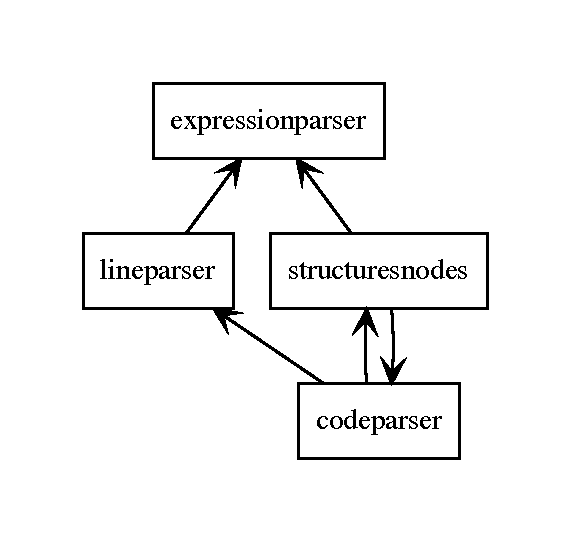
\includegraphics[scale=0.7]{./Pictures/parser.pdf}
	\captionof{figure}{}
\end{minipage}

\begin{figure}[h!]
	\centering
	\begin{tikzpicture}
	\node (ifelif) at (0,0) {
		\begin{minipage}{6cm}
		\inputminted[frame = single]{python}{example.code}
		\end{minipage}
	};
	
	
	\node[right = 4cm of ifelif.east] (ifelseif) {
\begin{minipage}{7.5cm}
\begin{minted}[frame = single]{text}
[<structuresnodes.AffectationNode >,
<structuresnodes.AffectationNode >,
<structuresnodes.WhileNode>,
<structuresnodes.PrintNode>]
\end{minted}
\end{minipage}
	};
	
	\draw[->] (ifelif.east) -- (ifelseif) node[midway, above] {\pyinline{CodeParser}};
	\end{tikzpicture}
	\caption{\label{fig:parse_exemple}Exemple simpliste de parse}
\end{figure}


\subsubsection{Classe CodeParser}

L'analyse du code est gérée par un objet de la classe \pyinline{CodeParser} dont le constructeur prend en argument:
\begin{itemize}
	\item soit un nom de fichier \pyinline{filename = file}
	\item soit une chaine de caractère contenant un fragment de code \pyinline{code = fragment}
\end{itemize}

Un objet de type \pyinline{CodeParser} a pour attributs:
\begin{itemize}
	\item \pyinline{__listingCode}: une liste d'objets de type \pyinline{LineParser}
	\item \pyinline{__structuredListeNode} un arbre d'objets de type StructureNode contenant le code interprété
\end{itemize}

Lorsque le code est donné sous forme de fichier, la méthode \pyinline{__parseFile} permet de récupérer la chaîne de caractères correspondante.

La méthode \pyinline{parseCode} construit une instance de la classe \pyinline{LineParser} pour chaque ligne de code source. Si la ligne n'est pas vide, les caractéristiques de celles-ci sont ajoutées à la liste \pyinline{__listingCode}.

Une analyse syntaxique succincte est réalisée avec l'appel successif aux méthodes:
\begin{itemize}
	\item  \pyinline{__manageElif()}: réécriture des branchements \pyinline{elif}).
	\begin{center}

\begin{tikzpicture}
\node (ifelif) at (0,0) {
\begin{minipage}{3cm}
\begin{minted}[frame = single]{python}
if e1 :
	c1
elif e2 :
	c2
else c3
\end{minted}
\end{minipage}
};


\node[right = 5cm of ifelif.east] (ifelseif) {
\begin{minipage}{5cm}
\begin{minted}[frame = single]{python}
if e1 :
	c1
else :
	if e2 :
		c2
	else :
		c3
\end{minted}
\end{minipage}
};

\draw[->] (ifelif.east) -- (ifelseif) node[midway, above] {\pyinline{__manageElif()}};
\end{tikzpicture}
		
	\end{center}
	\item \pyinline{__blocControl()}: test de la syntaxe des structures de contrôle et de l'indentation associée.
\end{itemize}


Finalement, la construction de l'arbre \pyinline{__structuredListeNode} nécessite l'appel des méthodes:
\begin{itemize}
	\item \pyinline{__buildFinalNodeList()}: construit les n\oe uds (instances de classe \pyinline{structuresnodes}) et l'arborescence correspondante à partir des caractéristiques \pyinline{__listingCode}. Les blocs d'instructions sont ajoutés à \pyinline{__structuredListeNode}.
	
	\item \pyinline{__structureList}: Parcours du listing \pyinline{__listingCode} pour ranger les enfants et leur associer le bon niveau d'indentation
\end{itemize} 


L'arborescence des n\oe uds \pyinline{__listingCode} peut-être affichée à l'aide des méthodes \pyinline{__str__()} et \pyinline{__recursiveStringifyLine()}.

L'accès à la liste de n\oe uds \pyinline{__structureList} est possible à l'aide de l'accesseur \pyinline{getFinalParse()}.

\subsubsection{Classe LineParser}

La classe \pyinline{LineParser} permet de renvoyer les caractéristiques d'une ligne de code sous forme d'un dictionnaire contenant numéro de ligne, niveau d'indentation, caractère vide ou non, motif identifié (if,....), condition, expression ou variable le cas échéant.

Pour une ligne de code donnée elle doit:
\begin{itemize}
	\item Nettoyer le code des commentaires et espaces terminaux: \pyinline{__suppCommentsAndEndSpaces()}
	\item Déterminer le niveau d'indentation: \pyinline{__countIndentation()}
	\item Pour les lignes non vides, identifier le motif: \pyinline{__identificationMotif()}
\end{itemize}

Lorsque le motif correspond à un branchement conditionnel \pyinline{if e} ou une boucle \pyinline{while e} l'identification du motif \pyinline{__identificationMotif()} nécessite de tester que \pyinline{e} est une expression valide. L'expression correspondante est construite par une instance de la classe \pyinline{ExpressionParser}.


\subsubsection{Classe ExpressionParser}

Les objets de la classe \pyinline{ExpressionParser}  permettent l'interprétation d'une chaine de caractère afin de renvoyer un objet de type \pyinline{Expression}, c'est à dire un arbre dont chaque n\oe ud représente un opérateur binaire, un opérateur unaire, une variable ou un littéral représentant l'expression en notation polonaise inverse.

Pour cela la chaine de caractère représentant l'expression est convertie en une liste de Tokens (\pyinline{__buildTokensList()}) représentant chaque type admissible dans la chaine de caractère. Ceux-ci peuvent correspondre à:
\begin{itemize}
	\item une variable \pyinline{TokenVariable}
	\item un nombre \pyinline{TokenNumber}
	\item un opérateur binaire \pyinline{TokenBinaryOperator}
	\item un opérateur unaire \pyinline{TokenUnaryOperator}
	\item une parenthèse \pyinline{TokenParenthesis}
\end{itemize}

La classe doit permettre de vérifier la syntaxe de l'expression:
\begin{itemize}
	\item \pyinline{strIsExpression()} s'assure que la chaîne de caractère est une expression régulière;
	\item \pyinline{testBrackets()} teste l'équilibre des parenthèses;
	\item \pyinline{__tokensListIsLegal()} teste si l'enchaînement de Token est correct à partir de la table de vérité (\ref{tab:TokenListLegal})
	\item \pyinline{__consolidAddSub()} doit permettre de simplifier la liste de Token pour des enchainements de type \pyinline{'(+'}, \pyinline{'+-'},...
\end{itemize}

\begin{table}[h!]
	\centering
	\caption{\label{tab:TokenListLegal}Enchainements autorisés de Token}
	\begin{tabular}{|L{3cm}|C{1.8cm}|C{1.8cm}|C{1.8cm}|C{1.8cm}|C{1.8cm}|C{1.8cm}|}
\hline
\diagbox[width=10em, height=2.8em]{\textbf{Précédent}}{\textbf{Suivant}}  & \textbf{None} & \textbf{Opérateur Binaire} & \textbf{Opérateur Unaire} & \textbf{Opérande} & \textbf{(} & \textbf{)} \\ \hline
\textbf{None}                & 1             & 0                            & 1                           & 1                 & 1          & 0          \\ \hline
\textbf{Opérateur Binaire} & 0             & 0                            & 1                           & 1                 & 1          & 0          \\ \hline
\textbf{Opérateur Unaire}  & 0             & 0                            & 0                           & 1                 & 1          & 0          \\ \hline
\textbf{Opérande}            & 1             & 1                            & 0                           & 0                 & 0          & 1          \\ \hline
\textbf{(}                   & 0             & 0                            & 1                           & 1                 & 1          & 0          \\ \hline
\textbf{)}                   & 1             & 1                            & 0                           & 0                 & 0          & 1          \\ \hline
\end{tabular}
\end{table}



A partir de la liste de Token, la construction de l'arbre associé à l'expression nécessite:
\begin{itemize}
	\item \pyinline{__buildReversePolishNotation()}: réorganisation de la liste de Token en notation polonaise inverse
	
	\begin{center}
		\begin{tikzpicture}
		\node (begin) at (0,0) {
			\begin{minipage}{4cm}
\begin{minted}[frame = single]{python}
(3 + 4) * 5 - 7 / 8
\end{minted}
			\end{minipage}
		};
		
		
		\node[right = 5cm of begin.east] (end) {
\begin{minipage}{4cm}
\begin{minted}[frame = single]{python}
3 4 + 5 * 7 8 / -
\end{minted}
\end{minipage}
		};
		
		\draw[->] (begin.east) -- (end) node[midway, above] {\pyinline{__buildReversePolishNotation}};
		\end{tikzpicture}
	\end{center}
\item \pyinline{__buildTree()}: construction de l'arbre associé à l'expression. Fait appel à la méthode \pyinline{toNode()} de la classe \pyinline{Token} pour créer les instances des classes \pyinline{ArithmeticExpressionNode}, \pyinline{ComparaisonExpressionNode} ou \pyinline{LogicExpressionNode} suivant le type d'expression analysée.
\end{itemize}

\subsubsection{Token}
Les classes \pyinline{TokenVariable}, \pyinline{TokenNumber}, \pyinline{TokenBinaryOperator}, \pyinline{TokenUnaryOperator} et \pyinline{TokenUnaryOperator} héritées de la classe \pyinline{Token} implémentent l'ensemble des tests nécessaires à l'identification et à l'usage des Token (gestion de priorité, distinction opérateurs/opérandes, etc...) 

\begin{figure}[h!]
	\centering
	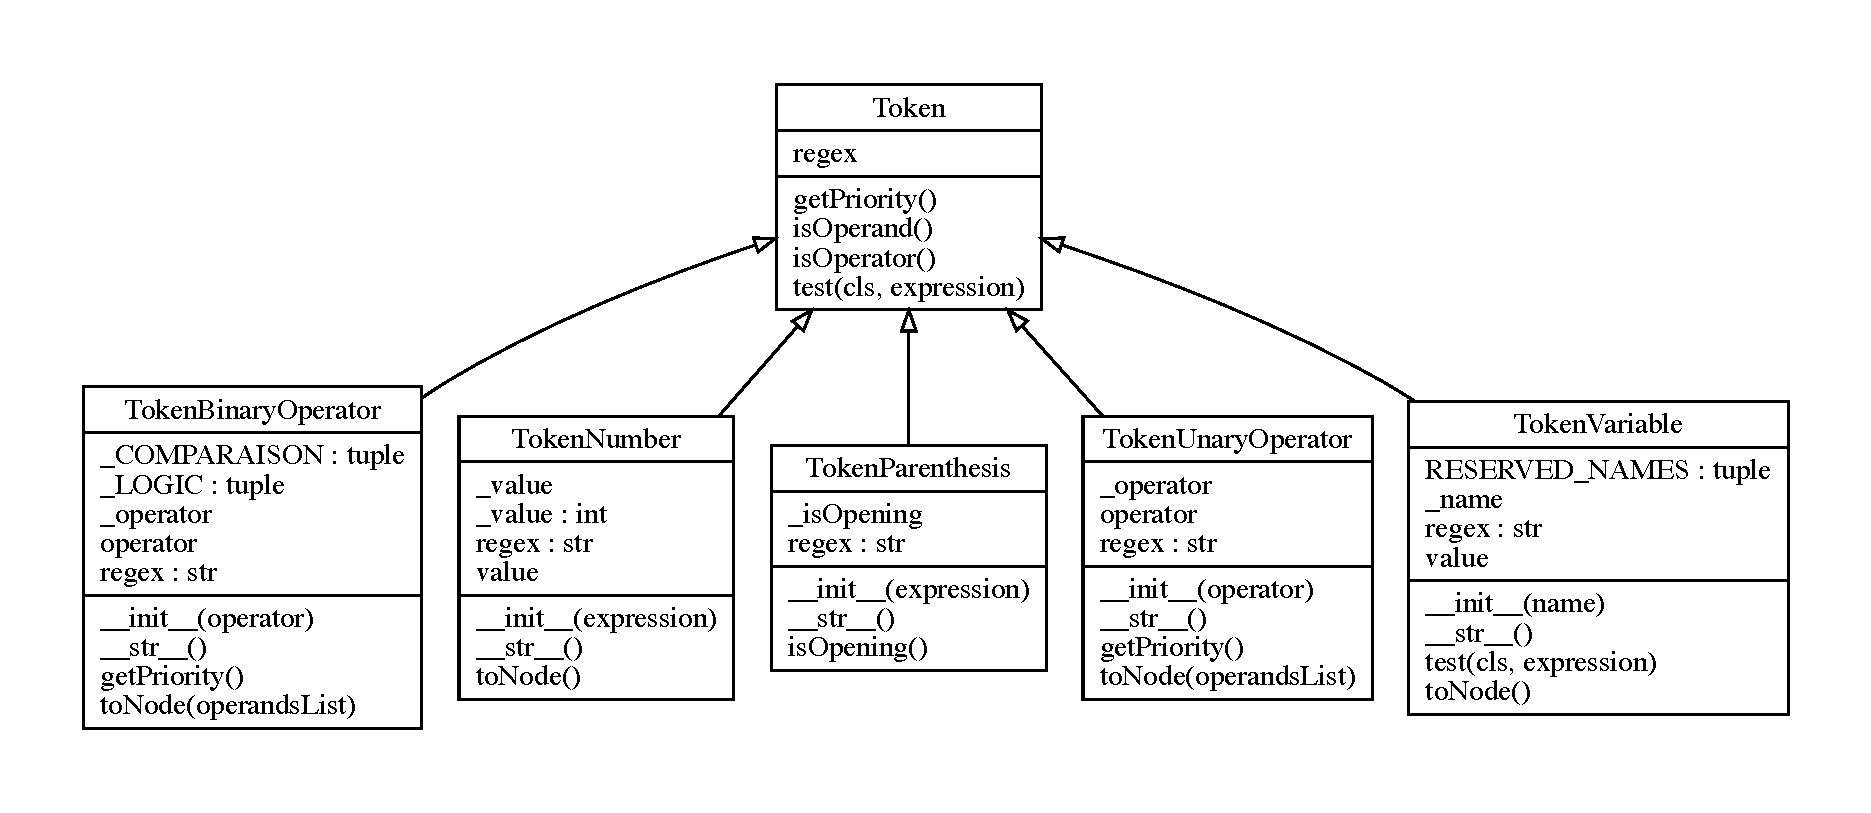
\includegraphics[width = 20cm]{./Pictures/Token.pdf}
	\caption{\label{fig:class_Token} Diagramme de classe Token}
\end{figure}